\documentclass{beamer}
\title{Git Basics}
\author{David Kouka}
\date{\today}

\usepackage{tikz}
\usetikzlibrary{automata}
\usetikzlibrary{arrows.meta, positioning, calc}
\usepackage{graphicx}   % For including images
\usepackage{listings}   % For code listings

\lstset{
    basicstyle=\ttfamily\color{blue}, % Change color and font
    keywordstyle=\color{red},
    commentstyle=\color{green},
    stringstyle=\color{orange},
    columns=flexible,
    keepspaces=true,
    showstringspaces=false,
}

\begin{document}

\frame{\titlepage}  % Title slide

\section{Table of Contents}

\begin{frame}
    \frame{Table of Contents}
    \tableofcontents
\end{frame}

\section{Version control}

\begin{frame}{Why using version control}
    \begin{itemize}
        \item<1-> Tracking changes \lstinline{git diff} Register
        \item<2-> Backup and recovery \lstinline{git checkout} Time machine
        \item<3-> Collaborative work (authors, conflicts, PR)
        \item<4-> Accountability \lstinline{git blame}
        \item<5-> "Documentation" via commit messages \lstinline{git log}
        \item<6-> Safe experiments \lstinline{git branch} *boum*
        \item<7-> Easy release management (tags, banches, CI/CD, ...)
    \end{itemize}
\end{frame}

\section{Git commands}

\begin{frame}{Hosting}
    \only<1-> Git hosting platforms
    \begin{itemize}
        \item<2-> Bitbucket 
\includegraphics[width=0.07\linewidth]{img/logo_bitbucket.png}
        \item<3-> Gitea 
\includegraphics[width=0.07\linewidth]{img/logo_gitea.png}
        \item<4-> Github 
\includegraphics[width=0.07\linewidth]{img/logo_github.png}
        \item<5-> Gitlab 
\includegraphics[width=0.07\linewidth]{img/logo_gitlab.png}
    \end{itemize}
\end{frame}

\subsection{Cloning}

\begin{frame}{git clone}
    \only<1-> Copy repository from server \pause
    \centering
    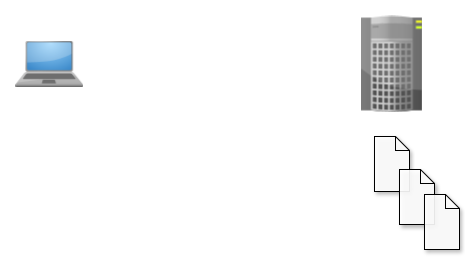
\includegraphics[width=0.8\linewidth]{img/git_clone_1.png}
\end{frame}
\begin{frame}{git clone}
    Copy repository from server 
    \centering
    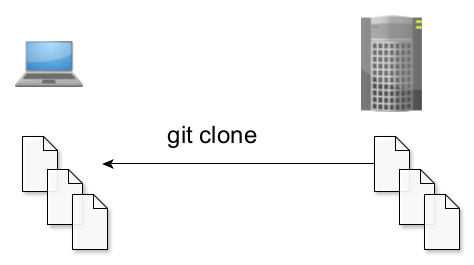
\includegraphics[width=0.8\linewidth]{img/git_clone_2.png}
\end{frame}

\subsection{Stage/Commit/Push}

\begin{frame}{git add}
    \centering
    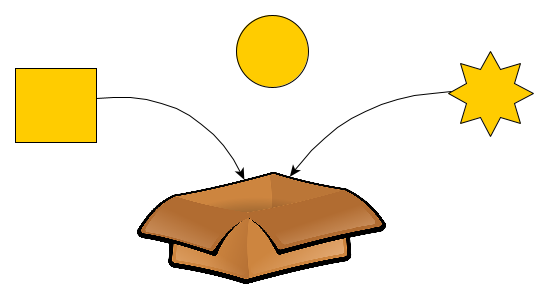
\includegraphics[width=0.7\linewidth]{img/git_add_1.png}
\end{frame}
\begin{frame}{git add}
    \centering
    
\includegraphics[width=0.7\linewidth]{img/git_add_2.png}
\end{frame}

\begin{frame}{git commit}
    \centering
    
\includegraphics[width=0.4\linewidth]{img/commit.png}
\end{frame}

\begin{frame}{git push}
    \centering
    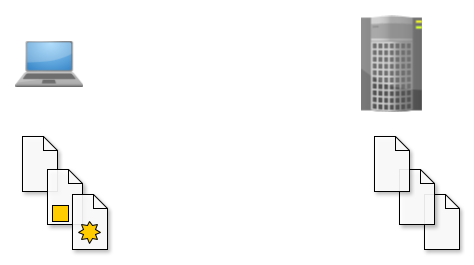
\includegraphics[width=0.7\linewidth]{img/git_push_1.png}
\end{frame}
\begin{frame}{git push}
    \centering
    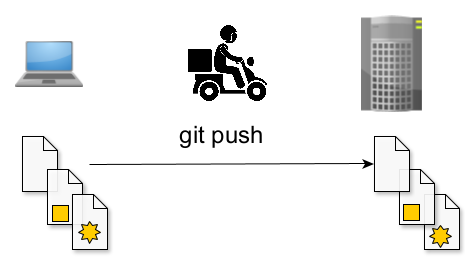
\includegraphics[width=0.7\linewidth]{img/git_push_2.png}
\end{frame}

\subsection{git branch}

\begin{frame}{git branch}
    \begin{tikzpicture}[
            node/.style={circle, draw=black, very thick, minimum size=15mm},
            img/.style={minimum size=15mm}
        ]

        % Step 1: Main branch
        \node[node] (main) {main};
        \node[img] (img1) [right=of main] {
\includegraphics[width=15mm]{img/bunshin.png}};
        
        \pause
        
        % Step 2: Branches
        \node[node] (rasengan) [below left=of main] {\small rasengan};
        \node[img] (img2) [left=of rasengan] {
\includegraphics[width=15mm]{img/rasengan.png}};
        
        \node[node] (senin) [below right=of main] {senin};
        \node[img] (img3) [right=of senin] {
\includegraphics[width=15mm]{img/sage.png}};

        % Arrows from main to branches
        \draw[->] (main) -- (rasengan) node[midway, left] {\texttt{git branch rasengan}};
        \draw[->] (main) -- (senin) node[midway, right] {\texttt{git branch senin}};

        \pause
        
        % Step 3: Merge
        \node[node] (merge) [below=of $(rasengan.south)!0.5!(senin.south)$] {merge};
        \node[img] (img4) [right=of merge] {
\includegraphics[width=15mm]{img/naruto_sage_rasengan.png}};
        
        \draw[->] (rasengan) -- (merge) node[midway, left] {\texttt{git merge}};
        \draw[->] (senin) -- (merge) node[midway, right] {\texttt{git merge}};
        
    \end{tikzpicture}
\end{frame}


%\subsection{Merge}


%\subsection{Conflicts}


\end{document}
